
Os resultados apresentados posteriormente foram gerados usando a base de dados KITTI \cite{Geiger}.

No primeiro teste na figura \ref{fig:imgpapercerta}, o algoritmo busca o objeto na sequ�ncia das
9 imagens com um deslocamento aproximadamente perpendicular em rela��o ao observador.

\begin{figure}[!hbt]
\centering
  \subfloat[]{\label{fig:imgpapercertaa} 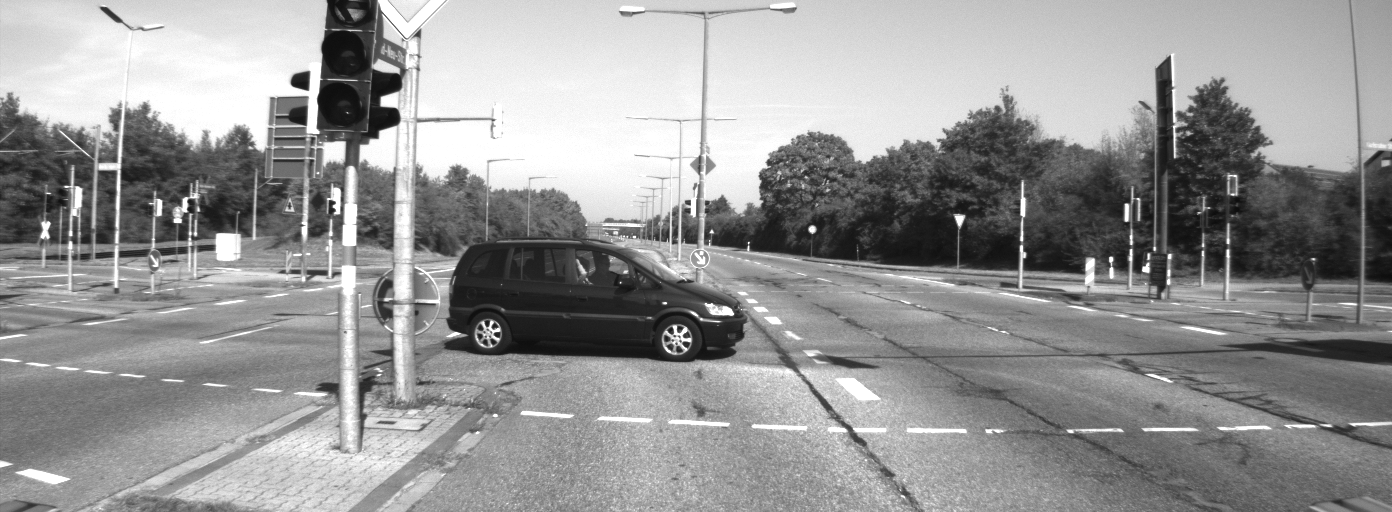
\includegraphics[width=.48\columnwidth]{images/images/0000000000.png}}
  \subfloat[]{\label{fig:imgpapercertab} 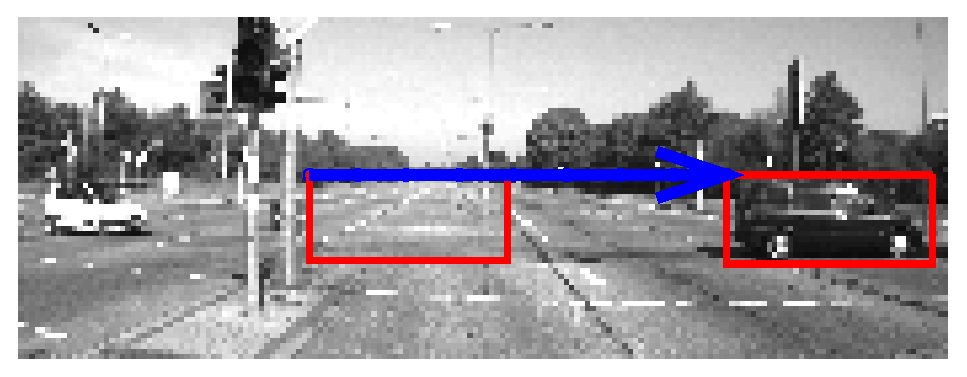
\includegraphics[width=.48\columnwidth]{images/images/img_paper_certa.eps}}
  \caption{A imagem (a) representa o objeto na sua posi��o inicial 
   e a imagem (b) mostra o ve�culo na posi��o final.}
  \label{fig:imgpapercerta}
\end{figure}

O vetor em azul ilustra o resultando da busca, saindo do ponto inicial at� o final. 
Nota-se, tamb�m, que existe uma curvatura na foto devido � c�mera e, por consequ�ncia,
um impacto no resultado. Deste modo, � poss�vel verificar a sensibilidade do algoritmo 
por menor que seja a varia��o da �rea do $ROI$, como mostrado na figura \ref{fig:res_graph1}.

\begin{figure}[!hbt]
\centering
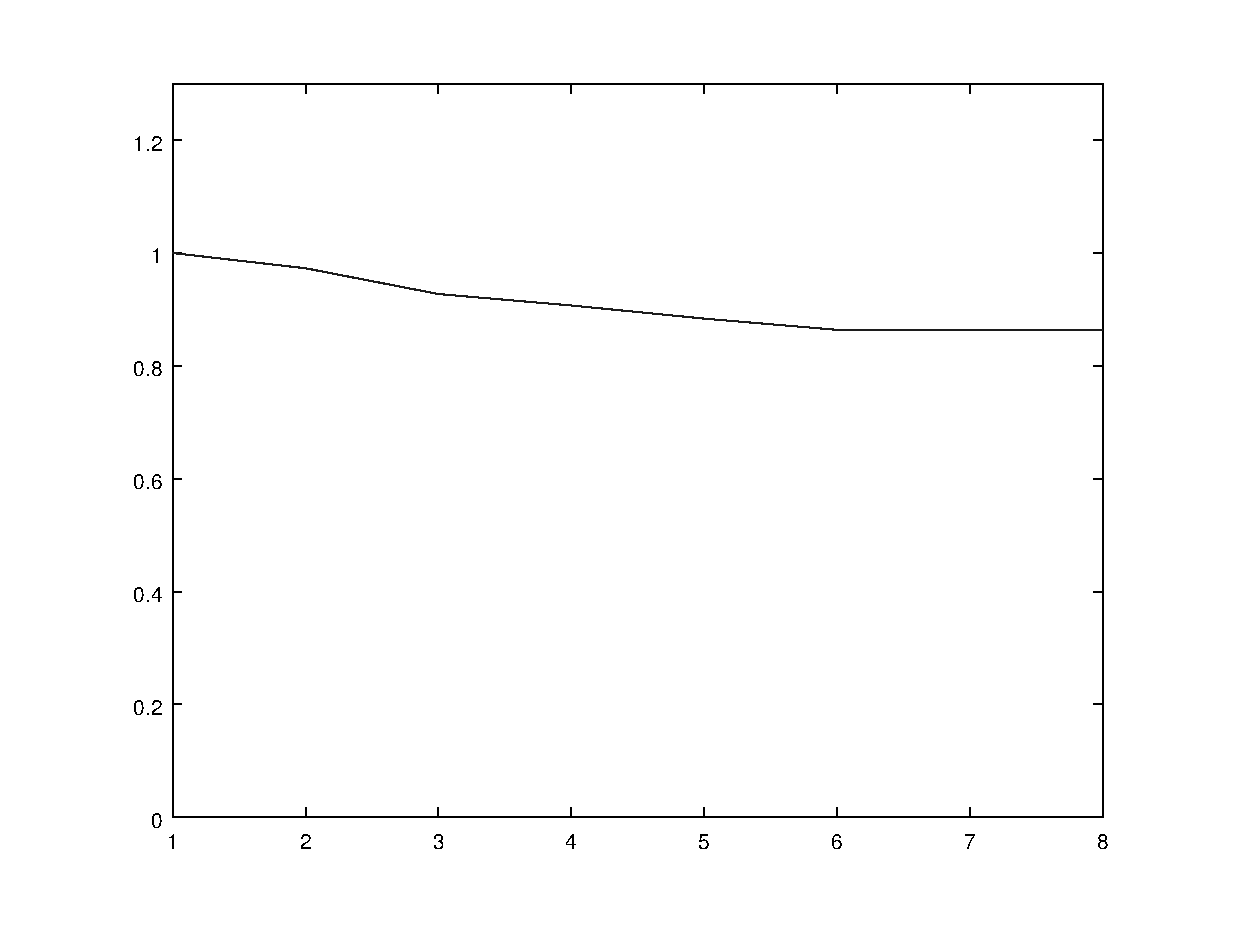
\includegraphics[width=0.8\columnwidth]{images/graph1.eps}
\caption{Fator de aproxima��o para cada imagem no teste 1.}
\label{fig:res_graph1}
\end{figure}

Na figura \ref{fig:res_graph1v} observa-se a velocidade com que o fator de aproxima��o se modifica e, ainda,
� poss�vel constatar a pequena varia��o no fator de aproxima��o, se comparado
com o valor de refer�ncia 1. A m�dia do fator de aproxima��o(velocidade) � de $-0.017020$, implicando
em uma aproxima��o de $1.7\%$ de $d_0$ em cada um das nove imagens.

\begin{figure}[!hbt]
\centering
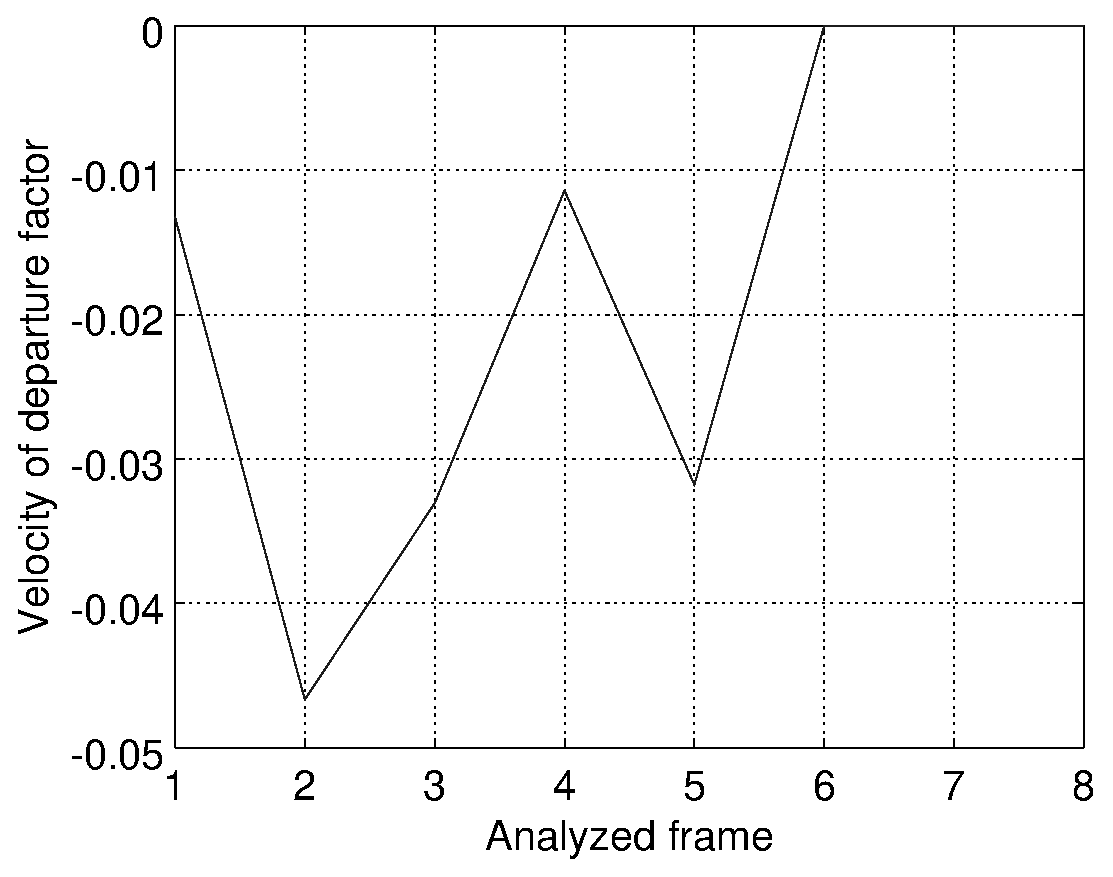
\includegraphics[width=0.8\columnwidth]{images/graph1v.eps}
\caption{Velocity of departure factor for each frame in the test 1.}
\label{fig:res_graph1v}
\end{figure}